\input{/home/herget/LMU/templates/solutions.tex}

\usepackage{natbib}
\usepackage{filecontents}
\usepackage{cleveref}
\bibliographystyle{plain}
\begin{filecontents}{\jobname.bib}
    @misc{BibEntry2013Dec,
    	title = {{{$<$}iterator{$>$} - C++ Reference}},
    	year = {2013},
    	month = {Dec},
    	note = {[Online; accessed 7. May 2018]},
    	url = {http://www.cplusplus.com/reference/iterator}
    }
\end{filecontents}

\newcommand{\hmwkTitle}{Assignment 03} % Assignment title
\newcommand{\hmwkClass}{CPPPC} % Course/class
\newcommand{\hmwkAuthorName}{Marius Herget} % Your name

\begin{document}
\maketitle\tableofcontents\newpage
\begin{homeworkProblem}[3-0: Prerequisites]
    \subsection{3-0-1: Iterator Concepts}
        \begin{itemize}
            \item Make yourself familiar with the Iterator concepts in the STL:
                \\\url{ http://en.cppreference.com/w/cpp/concept/Iterator}
            \item What are the differences between the concepts ForwardIterator and RandomAccessIterator?
                \problemAnswer{
                    \begin{itemize}
                        \item ForwardIterator reads and writes from the first element to the last element. Hence it follows the order of the data.
                        \item RandomAccessIterator read and writes obviously on random access. Hence it access data in a non-sequentially (via offsets).
                        \item As shown in \cref{itercat} there are different iterator categories. Input is the most restricted one. A ForwardIterator is way more restricted than the RandomAccessIterator.
                        \item A RandomAccessIterator have similiar functionality as standard pointers.
                        \item The detailed properties can be seen in the \textit{Iterator categories properties} table in \citep{BibEntry2013Dec}.
                    \end{itemize}
                }
                \begin{figure}[h!]
                    \begin{center}
                    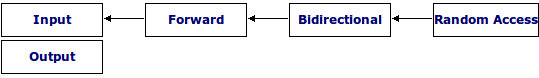
\includegraphics[width=0.75\textwidth]{img/itercat.png}
                    \caption{Iterator categories~\citep{BibEntry2013Dec}}
                    \label{itercat}
                \end{center}
                \end{figure}
            \item What are the differences between the concepts InputIterator and OutputIterator?
                \problemAnswer{
                    \begin{itemize}
                        \item Input- and OutputIterators are the most restricted Iterator categories. ''They can perform sequential single-pass input or output operation`` \citep{BibEntry2013Dec}.
                        \item An Input operation is comparable with an \texttt{istream / read} operation it it since gets something from the memory and makes it available to your program.
                        \item An Output operation in comparision puts something from your application back out into the environment (\texttt{write}).
                    \end{itemize}
                }
        \end{itemize}
    \subsection{3-0-2: Sequence Container Concept}
    Sequence containers implement data structures which can be accessed sequentially. Methods \texttt{begin()} and \texttt{end()} define the iteration space of the container elements.
    \begin{itemize}
        \item Make yourself familiar with Sequence Container concept defined in the STL: \\\url{http://en.cppreference.com/w/cpp/concept/SequenceContainer}
    \end{itemize}
    \note{Implement?!?}
    \textbf{Excerpt:}
    \begin{table}[h!]
        \label{tab:table1}
        \begin{tabular}{ll}
          \textbf {Type} & \textbf{Synopsis} \\
          \texttt{typename      value\_type}    &   the container’s element type T \\
          \texttt{typename        iterator}     &  	iterator type referencing a container element \\
          \texttt{typename  const\_iterator}    &  	typically defined as const \texttt{iterator} \\
          \texttt{typename       reference}     & 	type definition for \texttt{value\_type \&} \\
          \texttt{typename const\_reference}    &  	type definition for \texttt{const value\_type \&}
        \end{tabular}
    \end{table}
    \begin{table}[http]
        \label{tab:table2}
        \begin{tabularx}{\textwidth}{lX}
          \textbf {Signature} & \textbf{Synopsis} \\
          \texttt{iterator begin()}                 & Iterator referencing the first element in the container or \texttt{end()} if  container is empty\\
          \texttt{const\_iterator begin()  const}    & const iterator referencing the first element in the container or \texttt{end()} if container is empty\\
          \texttt{iterator end()}                   & iterator referencing past the final element in the container\\
          \texttt{const\_iterator end()    const}    & const iterator referencing past the final element in the container\\
          \texttt{size\_type size()        const}    & 	number of elements in the container, same as \texttt{end()} - \texttt{begin()}
        \end{tabularx}
    \end{table}
    % \note{Anmerkung: Aufgabe 1 wurde in der Übung nur mündlich besprochen. Lösungen hier können falsch sein.}
\end{homeworkProblem}
\begin{homeworkProblem}[3-1: List Container Template]
    \begin{enumerate}
        \item Complete the implementation of the List container template discussed in the last lab session.
        \begin{itemize}
            \item Remember that all template code must be implemented in headers!
            \item In your implementation, ensure that \texttt{List<T>} and \texttt{List<T>::iterator} satisfy \texttt{std::list<t>} and the STL iterator concepts, in particular iterator traits which are based on iterator tags.
        \end{itemize}
        \item Use the test suite of \texttt{Vector} you ported to C++ in assignment 2 to test your implementation of the \texttt{List} container.
        \note{
            \begin{itemize}
                \item Implement \texttt{push\_back}, \texttt{pop\_back}
                \item \texttt{bidirectional\_iterator}??? ->  Nope ForwardIterator is enough.
                \item Implement as \texttt{doubly linked list}?? -> single linked is enough
                \item Whole Container concept: \\\texttt{begin(), end(), size(),\\ not: max\_size(), empty(), swap()}
                \item testsuite implementation
                    \begin{itemize}
                        \item Which concepts to test?
                    \end{itemize}
            \end{itemize}
        }
    \end{enumerate}
\end{homeworkProblem}
\begin{homeworkProblem}[3-2 : Measurements<T> Class Template]
Assuming you run a series of benchmarks, each returning a measurement. At the end of the test series, the mean, median, standard deviation (sigma) and variance should be printed.\\
Implement the class template Measurements<T> representing a sequence container that allows to collect measurement data as single values and provides methods to obtain the mean, median, standard deviation and variance of the container elements.
    \note{
        \begin{itemize}
            \item Is using the List container recommended? $->$ use \texttt{std:vector<>}
            \item Doppelindex? How? -> .X assignment
            \item Calc \texttt{median}, \texttt{mean}, \texttt{varience} and \texttt{sigma} in runtime or at modification? $->$ egal aber kann man ja cachen
        \end{itemize}
    }
\paragraph{Measurements Container Concept}\\
In addition to the Sequence Container Concept:
    \begin{table}[http]
        \label{tab:table3}
        \begin{tabularx}{\textwidth}{lX}
          \textbf {Signature} & \textbf{Synopsis} \\
          \texttt{T median()             const}    & returns the median of the elements in the container or $0$ if the container is empty \\
          \texttt{double mean()          const}    & returns the mean of the elements in the container \\
          \texttt{double variance()      const}    & returns the population variance of the elements in the container\\
          \texttt{double sigma()         const}    & returns the standard deviation of the elements in the container
        \end{tabularx}
    \end{table}\\\newpage
\textbf{Example:}
\begin{lstlisting}[language=C++]
Measurements<int> m1;
m1.insert(10);
m1.insert(34);

m1.size(); // = 2

Measurements<double> m2;
std::vector<double> v({ 36, 37, 10 });
m2.insert(v.begin(), v.end());

m1.insert(m2.begin(), m2.end())

m1.size(); // = 5

int    median = m1.median();
double mean   = m1.mean();
double sdev   = m1.sigma();
double var    = m1.variance();
\end{lstlisting}

Define a class template \texttt{Measurements<T>} that satisfies the Sequence Container concept (\url{http://en.cppreference.com/w/cpp/concept/SequenceContainer}) and the Measurements Container concept defined above.

You may ignore the \texttt{emplace} methods for now.

The solution uses \texttt{std::vector} as a starting point, but you may use any underlying data structure in your implementation of \texttt{cpppc::Measurements<T>}.
\end{homeworkProblem}
\begin{homeworkProblem}[3-X: Improve Efficiency]
    \begin{itemize}
        \item Refactor your implementation of \texttt{Measurements<T>} such that all methods in the Measurements concept maintain constant computational complexity $O(c)$
        \item There are arithmetic solutions, possibly at the cost of numeric stability, and approaches focusing on the underlying data structure
    \end{itemize}
\end{homeworkProblem}


\bibliography{\jobname}
\end{document}
